\section{Generalized Reeb Orbits On Polytopes}\label{sec:generalized-reeb-orbits-polytopes}

The boundary of a polytope is not smooth, so the smooth Reeb vector field is
replaced by a differential inclusion. This section records the nonsmooth
Reeb-orbit language needed to pass from the minimum-action formulation to the
finite Haim--Kislev quadratic program.

\subsection{Definition}\label{subsec:generalized-reeb-orbits-polytopes-definition}

Let
\[
  K=\{x\in\mathbb{R}^4:\langle a_i,x\rangle\leq 1,\; i=1,\ldots,F\}
\]
be a full-dimensional polytope with \(0\in\operatorname{int}(K)\). We assume
that this \(H\)-representation is irredundant, so the facet corresponding to
\(a_i\) is
\[
  F_i=\{x\in K:\langle a_i,x\rangle=1\}.
\]
In this normalization the contact-normalized Reeb direction on \(F_i\) is
\begin{equation}\label{eq:generalized-reeb-facet-vector}
  R_i=2J_0a_i.
\end{equation}
Indeed \(R_i\) is tangent to \(F_i\), because
\(\langle a_i,J_0a_i\rangle=0\), and for \(x\in F_i\),
\[
  \lambda_0|_x(R_i)
  =\frac{1}{2}\langle -J_0R_i,x\rangle
  =\langle a_i,x\rangle
  =1.
\]

A \emph{generalized Reeb orbit} on \(K\) is a curve
\(\gamma\in W^{1,2}([0,T],\mathbb{R}^4)\) with \(T>0\),
\(\gamma(0)=\gamma(T)\), image contained in \(\partial K\), and
\begin{equation}\label{eq:generalized-reeb-inclusion}
  \dot{\gamma}(t)
  \in \operatorname{conv}\{R_i:\gamma(t)\in F_i\}
  \quad\text{for a.e. }t\in[0,T].
\end{equation}
This is the polytope form of the Hamiltonian inclusion
\(-J_0\dot{\gamma}\in\partial g_K^2(\gamma)\), translated into the
contact-normalized Reeb directions. Since every \(R_i\) in the active convex
hull satisfies \(\lambda_0(R_i)=1\) at \(\gamma(t)\), a generalized Reeb orbit
has
\[
  A(\gamma)=T.
\]

A generalized Reeb orbit is \emph{simple} if its periodic parametrization can
be started so that \(\dot{\gamma}\), after changing values at finitely many
breakpoints if necessary, is constant on finitely many intervals and each
constant value is one of the pure facet directions \(R_i\). In addition, each
facet direction occurs in one connected time interval, possibly not at all.
Thus a simple orbit uses pure facet directions rather than nontrivial convex
combinations, and it does not return to the same facet direction in separated
time intervals.


\subsection{Words, dwell times, and closure}
\label{subsec:generalized-reeb-orbits-polytopes-words}

The finite computation records a simple orbit by its facet directions, dwell
times, and starting point. We use the \emph{active-word convention}: the word
contains exactly the distinct facet directions that occur with positive
duration, and the base point is chosen at a velocity breakpoint. A cyclic word
\[
  \sigma=(\sigma_1,\ldots,\sigma_m)
\]
with distinct entries, together with dwell times \(\tau_k>0\) and a base point
\(b=\gamma(0)\), describes the velocity data
\[
  \dot{\gamma}(t)=R_{\sigma_k}
  \quad\text{for a time interval of length }\tau_k.
\]
Such data can represent a closed orbit only if the closing equation holds:
\begin{equation}\label{eq:generalized-reeb-closure}
  \sum_{k=1}^m \tau_k R_{\sigma_k}=0.
\end{equation}
Closure of the velocity polygon is only the closedness equation for the broken
path. To turn the word and dwell times into an actual simple Reeb orbit on
\(\partial K\), one must choose a base point \(b\) so that each segment lies on
its prescribed facet; this is the base-point recovery construction of
Lemma~\ref{lem:generalized-reeb-base-point-recovery}.

\begin{figure}[htbp]
  \centering
  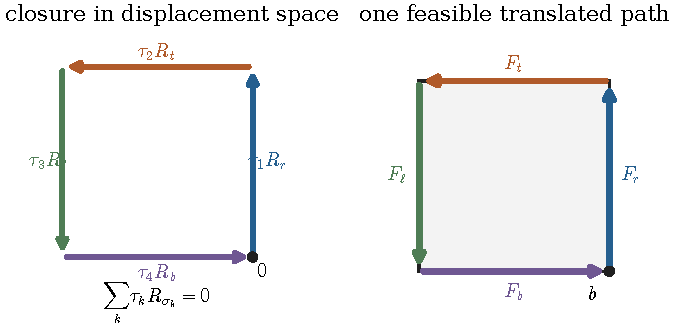
\includegraphics[width=0.94\linewidth]
    {figures/foundations/word-closure-basepoint.pdf}
  \caption{The two layers of finite orbit data in a two-dimensional
  Hamiltonian analogue.  The ordered displacements first form a closed
  velocity polygon.  A translation by a feasible base point then places every
  segment on its prescribed facet.  This is an exact planar example, not a
  projection of the four-dimensional orbit; it illustrates only closure and
  facet realizability.}
  \label{fig:generalized-reeb-word-closure-basepoint}
\end{figure}

Closure does not imply that the second layer is feasible.  For example, in the
planar square \([-1,1]^2\), the right and left facet rows give opposite
directions \(R_r=(0,2)\) and \(R_\ell=(0,-2)\).  Equal dwell times satisfy
\(\tau R_r+\tau R_\ell=0\), but the breakpoint between the two segments would
have to lie in the disjoint facets \(F_r\) and \(F_\ell\).  No translation can
realize this closed two-segment path on the prescribed facets.

The period and action of a closed pure-word orbit are
\[
  T=\sum_{k=1}^m \tau_k,
  \qquad
  A(\gamma)=T.
\]
This convention is the free-period convention used in
Theorem~\ref{thm:preliminaries-clarke-dual-action}.

The same geometric orbit has no preferred starting segment. Cyclically shifting
the \((\text{facet},\text{duration})\)-pairs gives the same orbit, provided the
base point is shifted to the corresponding breakpoint on the curve. If an orbit
is instead started inside a constant-velocity segment, that segment is split at
the start time and then merged again when the active word is recovered. If one
uses a padded convention with all facets in a permutation and dwell times
\(\tau_k\geq0\), then zero-duration entries are first deleted to recover the
active word.

The action of a finite word can be calculated directly from its velocities and
dwell times.

\begin{lemma}[Symplectic shoelace formula]\label{lem:preliminaries-shoelace}
Let \(z\colon[0,T]\to\mathbb{R}^4\) be a closed piecewise affine curve. Suppose
that \(z\) has constant velocity \(w_k\) on consecutive intervals of length
\(\ell_k\), for \(k=1,\ldots,m\). Then
\begin{equation}\label{eq:preliminaries-shoelace}
  2A(z)
  =
  \sum_{1\leq j<k\leq m}
    \ell_j\ell_k\,\omega_0(w_j,w_k).
\end{equation}
In particular, the action of a closed pure-word Reeb orbit depends only on the
cyclic velocity word and the dwell times, not on the base point.
\end{lemma}

\begin{proof}
Write \(t_k=\sum_{j<k}\ell_j\). On the \(k\)-th interval,
\[
  z(t)=z(0)+\sum_{j<k}\ell_jw_j+(t-t_k)w_k.
\]
The contribution of \(z(0)\) to
\(\int_0^T\langle -J_0\dot z,z\rangle\,dt\) vanishes because \(z\) is closed,
so \(\sum_k\ell_kw_k=0\). The self-term
\(\langle -J_0w_k,w_k\rangle\) vanishes by skew-symmetry. Hence
\[
  2A(z)
  =
  \sum_k
    \ell_k\left\langle -J_0w_k,\sum_{j<k}\ell_jw_j\right\rangle
  =
  \sum_{j<k}\ell_j\ell_k\,\omega_0(w_j,w_k),
\]
using \(\omega_0(u,v)=\langle J_0u,v\rangle\).
\end{proof}

Breakpoints of \(\dot{\gamma}\) are velocity changes, not necessarily changes
in the minimal face containing \(\gamma(t)\): an orbit may move inside a
nonsmooth face while switching from one active facet direction to another.

\begin{lemma}[Base-point recovery]\label{lem:generalized-reeb-base-point-recovery}
Fix an active word \(\sigma=(\sigma_1,\ldots,\sigma_m)\) and dwell times
\(\tau_k>0\) satisfying the closure equation
\eqref{eq:generalized-reeb-closure}. Put
\[
  v_1=0,
  \qquad
  v_k=\sum_{j=1}^{k-1}\tau_jR_{\sigma_j}
  \quad (k=2,\ldots,m+1).
\]
Then \(v_{m+1}=0\). A point \(b\in\mathbb{R}^4\) recovers a simple Reeb orbit
with these velocity data, by
\[
  \gamma(t)=b+v_k+sR_{\sigma_k},
  \qquad 0\leq s\leq \tau_k
\]
on the \(k\)-th segment, if and only if
\begin{equation}\label{eq:generalized-reeb-base-point-equalities}
  \langle a_{\sigma_k}, b+v_k\rangle=1
  \quad\text{for }k=1,\ldots,m,
\end{equation}
and
\begin{equation}\label{eq:generalized-reeb-base-point-inequalities}
  \langle a_i,b+v_k\rangle\leq 1
  \quad\text{for }i=1,\ldots,F\text{ and }k=1,\ldots,m.
\end{equation}
Equivalently, the equalities have the form
\[
  N_\sigma b = r_\sigma,
  \qquad
  (N_\sigma)_{k\bullet}=a_{\sigma_k}^{\mathsf T},
  \qquad
  (r_\sigma)_k=1-\langle a_{\sigma_k},v_k\rangle .
\]
When this system is nonempty, its solution space is an affine space of
dimension \(4-\operatorname{rank}N_\sigma\). The inequalities cut out the
valid base points as a convex polytope inside this affine space. In particular,
the set of valid base points is bounded, because \(v_1=0\) and
\eqref{eq:generalized-reeb-base-point-inequalities} imply \(b\in K\).
\end{lemma}

\begin{proof}
On the \(k\)-th segment, the prescribed facet equation is
\[
  \langle a_{\sigma_k}, b+v_k+sR_{\sigma_k}\rangle=1.
\]
The \(s\)-term vanishes because
\(\langle a_{\sigma_k},R_{\sigma_k}\rangle
=2\langle a_{\sigma_k},J_0a_{\sigma_k}\rangle=0\). Hence the whole segment
lies on \(F_{\sigma_k}\) exactly when
\eqref{eq:generalized-reeb-base-point-equalities} holds.

The segment lies in \(K\) exactly when
\[
  \langle a_i,b+v_k+sR_{\sigma_k}\rangle\leq 1
  \quad\text{for all }i\text{ and all }s\in[0,\tau_k].
\]
For fixed \(i,k\) this expression is affine in \(s\), so it is enough to check
the endpoints. The endpoint at \(s=0\) is \(b+v_k\), and the endpoint at
\(s=\tau_k\) is \(b+v_{k+1}\). As \(k\) runs cyclically and \(v_{m+1}=v_1=0\),
these endpoint checks are exactly
\eqref{eq:generalized-reeb-base-point-inequalities}. With these equalities and
inequalities, the resulting closed broken path lies on \(\partial K\) and has
velocity \(R_{\sigma_k}\) on the \(k\)-th segment, hence is a simple Reeb orbit
with the prescribed data.
\end{proof}

\begin{remark}[Non-uniqueness and computation]
The base point is not part of the finite action data. If
\(\operatorname{rank}N_\sigma=4\), the facet equations determine it uniquely
when they are consistent. If \(\operatorname{rank}N_\sigma<4\), the inequalities
may leave a positive-dimensional set of base points. This non-uniqueness does
not affect the action, which is determined by the closed velocity polygon via
Lemma~\ref{lem:preliminaries-shoelace}. Computationally, base-point recovery is
therefore a finite linear feasibility check after the word and dwell times have
been chosen.
\end{remark}

\subsection{Existence of simple minimizers}
\label{subsec:generalized-reeb-orbits-polytopes-existence-of-simple-minimizers}

Haim--Kislev prove that every convex polytope has a minimum-action generalized
Reeb orbit with a simple finite description \cite[Theorem~1.5]{HK2017}. In
their statement the velocities are positive multiples of \(J_0n_i\) for the
unit facet normals \(n_i\). Here we reparametrize each segment by its
contact-normalized facet direction \(R_i=2J_0a_i\), absorbing the positive
multiples into the dwell times. The proof is important for the finite
computation, so we record the argument in the conventions of this thesis. It
starts from an arbitrary minimizer, passes to the dual formulation from
Theorem~\ref{thm:preliminaries-clarke-dual-action}, and constructs simpler
dual curves whose values converge back to the minimum.

\begin{theorem}[Simple minimizer]\label{thm:generalized-reeb-simple-minimizer}
Let \(K\subset\mathbb{R}^4\) be a full-dimensional convex polytope with
\(0\in\operatorname{int}(K)\). Among all generalized Reeb orbits on
\(\partial K\), there exists a minimum-action orbit that is simple in the
contact-normalized convention above. Hence
\[
  c_{\mathrm{EHZ}}(K)
  =
  \min\{A(\gamma):\gamma
  \text{ is a simple Reeb orbit on }\partial K\}.
\]
\end{theorem}

The proof uses five elementary operations on dual curves. The first operation
replaces a \(W^{1,2}\)-curve by a piecewise affine one.

\begin{lemma}[Piecewise affine approximation]\label{lem:generalized-reeb-pw-affine-approx}
Let \(z\in W^{1,2}([0,T],\mathbb{R}^4)\) be closed and satisfy
\[
  \dot z(t)\in\operatorname{conv}\{R_1,\ldots,R_F\}
  \quad\text{for a.e. }t.
\]
For every \(\varepsilon>0\), there is a closed piecewise affine curve \(z'\)
with
\[
  \dot z'(t)\in\operatorname{conv}\{R_1,\ldots,R_F\}
\]
on each affine piece and \(\|z'-z\|_{W^{1,2}}<\varepsilon\). Consequently
\(A(z')\to A(z)\) and \(I_K(z')\to I_K(z)\) as \(\varepsilon\to0\).
\end{lemma}

\begin{proof}
Let \(C=\operatorname{conv}\{R_1,\ldots,R_F\}\). Conditional expectations onto
refining finite partitions converge to \(\dot z\) in \(L^2\). Choose one such
partition \(0=t_0<\cdots<t_m=T\) so that the conditional averages of
\(\dot z\) on the partition intervals are \(L^2\)-close to \(\dot z\). On
\([t_k,t_{k+1}]\), put
\[
  w_k=\frac{1}{t_{k+1}-t_k}\int_{t_k}^{t_{k+1}}\dot z(s)\,ds.
\]
Because \(C\) is convex and closed, each \(w_k\) lies in \(C\). Define \(z'\)
by \(z'(0)=z(0)\) and \(\dot z'=w_k\) on \([t_k,t_{k+1}]\). Then
\[
  z'(T)-z'(0)=\int_0^T\dot z'(t)\,dt=\int_0^T\dot z(t)\,dt=0,
\]
so \(z'\) is closed. Since \(\dot z'\to\dot z\) in \(L^2\), integration gives
\(z'\to z\) uniformly, hence in \(W^{1,2}\). The convergence of \(A\) follows
from bilinearity in \((z,\dot z)\), and the convergence of \(I_K\) follows
from continuity of \(h_K^2\) on the bounded velocity set.
\end{proof}

\begin{lemma}[Splitting mixed velocities]\label{lem:generalized-reeb-splitting}
Let \(z\) be a closed piecewise affine curve of period \(T\) whose velocities
lie in \(\operatorname{conv}\{R_1,\ldots,R_F\}\). Then there is a closed
piecewise affine curve \(z'\), with the same period, whose velocity on each
segment is one pure Reeb vector \(R_i\), such that \(A(z')\geq A(z)\) and
\[
  I_K(z')=T.
\]
\end{lemma}

\begin{proof}
On a segment with velocity \(v=\sum_i\theta_iR_i\), \(\theta_i\ge0\) and
\(\sum_i\theta_i=1\), replace the segment by subsegments with velocities
\(R_i\) and lengths \(\theta_i\) times the original length. The total
displacement and period are unchanged. The only change in the action is the
sum of the new internal cross-terms from
Lemma~\ref{lem:preliminaries-shoelace}. Reversing the order of the inserted
subsegments changes the sign of this internal contribution, so one of the two
orders does not decrease the action.

For a pure Reeb velocity \(R_i=2J_0a_i\),
\[
  -J_0R_i=2a_i,
  \qquad
  h_K(-J_0R_i)=2h_K(a_i)=2,
\]
because \(F_i\neq\varnothing\) and \(\max_{x\in K}\langle a_i,x\rangle=1\).
Thus \(h_K^2(-J_0R_i)=4\) on every pure segment, and
\[
  I_K(z')=\frac14\int_0^T4\,dt=T.
\]
\end{proof}

\begin{lemma}[Merging repeated velocities]\label{lem:generalized-reeb-merging}
Let \(z\) be a closed piecewise affine curve whose velocity on each segment is
one of the \(R_i\). If some \(R_i\) occurs in two non-adjacent segments, then
there is a rearrangement \(z'\) that merges those two occurrences into one
contiguous segment and satisfies
\[
  A(z')\geq A(z),
  \qquad
  I_K(z')=I_K(z).
\]
Repeating this operation, and merging adjacent equal-velocity intervals,
gives a closed piecewise affine curve in which each pure Reeb vector occurs in
at most one interval. Here adjacency is understood cyclically, since the curve
is closed.
\end{lemma}

\begin{proof}
Suppose a velocity \(v\) occurs in two segments \(I_r\) and \(I_s\), with
middle segments \(M=\{r+1,\ldots,s-1\}\). Merging \(I_s\) forward into \(I_r\)
changes only the action terms involving \(v\) and the middle velocities, and
the change is
\[
  \Delta A_{\mathrm{fwd}}
  =
  |I_s|\sum_{i\in M}|I_i|\,\omega_0(v,w_i).
\]
Merging \(I_r\) backward into \(I_s\) gives
\[
  \Delta A_{\mathrm{bwd}}
  =
  -|I_r|\sum_{i\in M}|I_i|\,\omega_0(v,w_i).
\]
The two changes have opposite signs, or both vanish, so one merge has
nonnegative action change. Closure is preserved because the multiset of
velocity-duration pairs is unchanged, and \(I_K\) is unchanged because it
depends only on the velocities and their durations.
\end{proof}

\begin{lemma}[Rescaling]\label{lem:generalized-reeb-rescaling}
Let \(z\) be a closed piecewise affine curve with pure Reeb velocities and
period \(T\). If all durations are multiplied by \(\beta>0\), the resulting
curve \(z'\) satisfies
\[
  A(z')=\beta^2A(z),
  \qquad
  I_K(z')=\beta I_K(z).
\]
\end{lemma}

\begin{proof}
In Lemma~\ref{lem:preliminaries-shoelace}, every action term contains a
product of two durations, so \(A\) scales by \(\beta^2\). The integrand in
\(I_K\) is unchanged and the time intervals are all multiplied by \(\beta\), so
\(I_K\) scales by \(\beta\).
\end{proof}

\begin{lemma}[Compactness of simple dual curves]\label{lem:generalized-reeb-compactness}
Let \(z_n\) be closed simple piecewise-Reeb curves whose periods satisfy
\(T_n\to T>0\). After translating the curves and passing to a subsequence,
\(z_n\) converges to a closed simple piecewise-Reeb curve \(z_*\) with period
\(T\), and
\[
  A(z_*)=\lim_n A(z_n),
  \qquad
  I_K(z_*)=T.
\]
\end{lemma}

\begin{proof}
Choose the initial point of each periodic curve at a breakpoint, and insert
zero dwell times for unused facet directions. Each curve is then determined up
to translation by a permutation of the finitely many facet directions, dwell
times in the simplex of total mass \(T_n\), and its period. Since
the periods eventually lie in a compact interval \([T/2,2T]\), a subsequence of
these finite-dimensional data converges. Translating the starting points gives
uniform convergence after identifying each domain with \([0,1]\) by linear
time rescaling. Closure passes to the limit because
\(\sum_i\tau_iR_{\sigma(i)}=0\) for every curve. Some limiting dwell times may be zero; deleting
those zero-duration entries recovers the active word of the limiting simple
curve. The action is continuous in the dwell-time data by
Lemma~\ref{lem:preliminaries-shoelace}. Since the remaining positive-duration
segments still have pure Reeb velocities, the same computation as in
Lemma~\ref{lem:generalized-reeb-splitting} gives \(I_K(z_*)=T\).
\end{proof}

\begin{proof}[Proof of Theorem~\ref{thm:generalized-reeb-simple-minimizer}]
Choose a capacity-realizing generalized Reeb orbit \(\gamma\). By
Theorem~\ref{thm:preliminaries-clarke-dual-action}, \(\gamma\) is also a dual
minimizer in the thesis convention, with
\[
  I_K(\gamma)=A(\gamma)=T=c_{\mathrm{EHZ}}(K).
\]
Moreover \(\dot\gamma(t)\in\operatorname{conv}\{R_1,\ldots,R_F\}\) for almost
every \(t\).

Apply Lemma~\ref{lem:generalized-reeb-pw-affine-approx} to approximate
\(\gamma\) by closed piecewise affine dual curves \(z_1\) with velocities in
the convex hull of the \(R_i\). Then apply
Lemma~\ref{lem:generalized-reeb-splitting} to obtain a closed pure-velocity
curve \(z_2\) with \(A(z_2)\geq A(z_1)\) and \(I_K(z_2)=T\). Apply
Lemma~\ref{lem:generalized-reeb-merging} to obtain a closed pure-velocity curve
\(z_3\) in which each \(R_i\) occurs at most once, still with
\[
  A(z_3)\geq A(z_2),
  \qquad
  I_K(z_3)=T.
\]
We take the initial approximation close enough that \(A(z_1)>T/2\); then
\(A(z_3)>0\). Now rescale all durations by
\[
  \beta=\frac{T}{A(z_3)}.
\]
The rescaled curve \(z_4\) satisfies
\[
  A(z_4)=\frac{T^2}{A(z_3)},
  \qquad
  I_K(z_4)=\frac{T^2}{A(z_3)}.
\]
Thus \(z_4\) is feasible for the dual problem with period \(T^2/A(z_3)\).
Since \(\gamma\) was a dual minimizer, \(I_K(z_4)\geq T\), and therefore
\(A(z_3)\leq T\). On the other hand \(A(z_3)\geq A(z_1)\), and
\(A(z_1)\to T\). Hence \(A(z_3)\to T\), the rescaling factors tend to \(1\),
and the periods of \(z_4\) tend to \(T\).

By Lemma~\ref{lem:generalized-reeb-compactness}, a subsequence of the \(z_4\)
converges up to translation to a closed simple piecewise-Reeb curve \(z_*\)
with \(A(z_*)=T\) and \(I_K(z_*)=T\). This curve is a dual minimizer. Applying
Theorem~\ref{thm:preliminaries-clarke-dual-action} again gives a
contact-normalized generalized Reeb orbit on \(\partial K\) in the same
translate/rescale family. In the reconstruction part of that theorem, the
corresponding characteristic has the form
\[
  t\longmapsto c\,z_*(t/c^2)+b/c
\]
for some \(c>0\), with
\[
  c^2=\nu=\frac{I_K(z_*)}{T}=1
\]
by \eqref{eq:preliminaries-dual-multiplier-value}. Thus the reconstruction
only translates \(z_*\). Its velocities
remain the pure facet directions \(R_i\), each used in one connected interval,
so the resulting orbit is simple and has minimum action.
\end{proof}

The theorem proves existence of at least one simple capacity minimizer. It is
not a classification of all minimum-action generalized Reeb orbits. Other
minimizers may pass through nonsmooth faces and may use convex combinations of
active facet directions. Thus the finite Haim--Kislev quadratic program is
justified as a capacity search because its search family contains a simple
capacity minimizer, not because every minimizer or every word has this form.
Infeasible words and duplicate descriptions can still occur.

\subsection{CH2021 smoothings and limits}
\label{subsec:generalized-reeb-orbits-polytopes-ch2021}

Chaidez--Hutchings study a different finite model for four-dimensional
polytopes, designed to compare Reeb dynamics on a polytope with Reeb dynamics
on smoothings of that polytope \cite{CH2021}. Their main hypotheses and
conclusions are not the same as the Haim--Kislev formula above. The
Haim--Kislev formula applies to convex polytopes in all even dimensions and
computes the EHZ capacity by a finite quadratic program. The
Chaidez--Hutchings construction is four-dimensional and uses a
\emph{symplectic polytope} hypothesis, which in particular excludes
Lagrangian two-faces so that the relevant combinatorial Reeb direction is
one-dimensional.

For such a four-dimensional polytope, a Chaidez--Hutchings combinatorial Reeb
orbit is a cyclic sequence of oriented line segments in the boundary. Each
segment lies in a face and points in the corresponding one-dimensional Reeb
cone. They distinguish three types. Type~1 orbits avoid the one-skeleton,
Type~2 orbits meet the one-skeleton only at finitely many segment endpoints,
and Type~3 orbits contain a bad one-face. The symplectic flow graph records
the Type~1 case: vertices are two-faces, edges are Reeb passages through
three-faces, and periodic graph orbits correspond to Type~1 combinatorial Reeb
orbits with the same action \cite[Proposition~2.2]{CH2021}.

The limit results in \cite{CH2021} explain why this combinatorial model is
useful for capacity computations on four-dimensional symplectic polytopes.
First, a nondegenerate Type~1 combinatorial Reeb orbit gives nearby Reeb orbits
on sufficiently small smoothings; their actions converge, while the rotation
number and Conley--Zehnder index agree with the combinatorial values for all
sufficiently small smoothing parameters \cite[Theorem~1.8]{CH2021}. Conversely,
given Reeb orbits on \(\partial X_{\varepsilon_i}\) with
\(\varepsilon_i\to0\) and uniformly bounded rotation number, a subsequence
converges to a Type~1 or Type~2 combinatorial Reeb orbit, again with action
convergence \cite[Theorem~1.9]{CH2021}. Combining this with the fact that an
EHZ-capacity minimizer can be chosen with rotation number at most \(2\), they
obtain a capacity formula for four-dimensional symplectic polytopes: minimize
over Type~2 combinatorial Reeb orbits and over Type~1 combinatorial Reeb orbits
with combinatorial rotation number at most \(2\), subject in both cases to
their finite-segment bound \cite[Corollary~1.13]{CH2021}.

This thesis uses these statements as background for the later flow-graph
section, not as a replacement for the Haim--Kislev quadratic program. The
current QP checkpoint uses the Haim--Kislev formula as the capacity interface.
The flow-graph algorithm based on CH2021, including its implemented scope and
its unsupported cases, is treated separately in
Section~\ref{sec:flow-graph-algorithm-ch2021}.

